\section{System Design}

\subsection{Functional Requirements}
The Student Life Support Service is designed to fulfill the specific functional requirements of three key user roles: Students, Dormitory Staff (or Student Affairs), and Administrators. Each role has its own set of features tailored to its needs within the system.

\noindent \textbf{User Type}: S-Student, DS-Dormitory Staff/Student Affairs, A-Admin (Operator) \\
\textbf{Categorized}: F-Functional, NF-Nonfunctional

\newcolumntype{L}{>{\arraybackslash}m{3.5cm}}
\begin{longtable}{|m{0.6cm}|m{2.8cm}|m{5.4cm}|m{1.6cm}|m{1.5cm}|m{1.8cm}|}
	\hline
	\textbf{No} & \textbf{Requirement }             & \textbf{Description}                                                                                          & \textbf{Priority} & \textbf{User Type}  & \textbf{Category} \\ \hline
	\endhead
	1  & Manage personal info     & Users can view and update their personal information.                                                 & Medium   & S, DS, A   & F           \\ \hline
	2  & Support tickets          & Users can create (raise), view support tickets.                                                       & High     & S, DS, A   & F           \\ \hline
	3  & Contact through messages & Users can contact the staff or students handling the support ticket through text messages.            & High     & S, DS      & F           \\ \hline
	4  & Ticket rating            & Students can rate their tickets which are marked as done.                                             & Medium   & S          & F           \\ \hline
	5  & View newsfeed            & Users can view a newsfeed of public pending/in-process tickets.                                        & Low      & S, DS, A   & F           \\ \hline
	6  & View notifications       & Users can view notifications and announcements.                                                       & Medium   & S, DS, A   & F           \\ \hline
	7  & Feedback and suggestions & Users can give feedback and suggestions for the system.                                                & Medium   & S, DS, A   & F          \\ \hline
	8  & Handle support tickets   & Dormitory staff can view and handle (mark as done, cancel) support tickets.                            & High     & DS         & F           \\ \hline
	9  & View past tickets        & Dormitory staff can view all previously handled support tickets.                                       & Medium   & DS         & F           \\ \hline
	10 & Manage notifications     & Dormitory staff and admins can create and manage notifications and announcements.                      & High     & DS, A      & F           \\ \hline
	11 & Manage users             & Admins can manage all users/roles (create, view, update, delete).                                      & High     & A          & F           \\ \hline
	12 & Manage tickets           & Admins can manage all support tickets (view, delete).                                                  & High     & A          & F           \\ \hline
	13 & Manage dormitories       & Admins can manage all dormitories (create, view, delete).                                              & Medium   & A          & F           \\ \hline
	14 & Manage system logs       & Admins can manage system logs (view, delete).                                                          & Medium   & A          & F           \\ \hline
	15 & Manage feedback          & Admins can manage system feedback (view, delete).                                                      & Low      & A          & F           \\ \hline
	16 & View system report       & Admins can generate and view system reports.                                                           & High     & A          & F           \\ \hline
	
	
	\caption{Functional Requirements}
	\label{tab:functionalRequirement}
\end{longtable}


For clearer comprehension, the table presented below provides a detailed visualization of the functional requirements, organized according to the different user roles within the system. This structure allows for a more precise understanding of how each role interacts with the system's features and capabilities.

\begin{longtable}{{|m{4.8cm}|m{12cm}|}} 
	\hline
	\textbf{User roles} & \textbf{Functional Requirements}\\ \hline
	\endhead
	
	Student & 	
	\begin{itemize}
		\item can view, update his/her personal information.
		\item can create (raise), view his/her support tickets. 
		\item can contact the staff who handles the support ticket through text messages.
		\item can rate his/her tickets which are marked as done.
		\item can view newsfeed (public pending/in process tickets).
		\item can view notifications, announcement.
		\item can give feedback and suggestions for the system.
	\end{itemize}
	
	\\ \hline
	
	Dormitory staff/ Student Affairs & 	
	\begin{itemize}
		\item can view, update his/her personal information.
		\item can view all available support tickets.
		\item can handle support tickets. (mark as done, cancelled)
		\item can view all past handled tickets.
		\item can contact students who owns the ticket through text messages.
		\item can view newsfeed (public pending/in process tickets).
		\item can create, view notifications, announcement. 
		\item can give feedback and suggestions for the system.
	\end{itemize}
	
	\\ \hline
	
	
	Admin (Operator) & 	
	\begin{itemize}
		\item can manage his/her personal information (view, update).
		\item can manage all users/roles (create, view, update, delete).
		\item can manage all support tickets (view, delete).
		\item can manage all dormitories (create, view, delete).
		\item can manage system logs (view, delete).
		\item can manage system feedback (view, delete).
		\item can view newsfeed (public pending/in process tickets).
		\item can manage notifications, announcement (create, view). 
		\item can view the system report.
	\end{itemize}
	
	\\ \hline
	
	
	\caption{Functional Requirements by User Roles} % needs to go inside longtable environment
	\label{tab:functionalRequirements}
\end{longtable}



\subsection{Non-Functional Requirements}
\noindent \textbf{Categorized}: NF-Nonfunctional

\newcolumntype{L}{>{\arraybackslash}m{3.5cm}}



	\begin{longtable}{|m{0.5cm}|m{2.5cm}|m{7cm}|m{1.5cm}|m{1.7cm}|m{2.4cm}|}
		\hline
		\textbf{No} & \textbf{Requirement}                & \textbf{Description}                                                                                                                               & \textbf{Priority} & \textbf{Category}  & \textbf{Functioning} \\ \hline
		\endhead
		1  & Fast Response Time          & The system should provide fast responses for user interactions such as submitting tickets, viewing statuses, and real-time messaging.      & High     & NF        & Performance \\ \hline
		2  & Real-Time Communication     & Messages between students and staff should be transmitted with minimal latency (under 100 milliseconds).                                   & High     & NF        & Performance \\ \hline
		3  & Concurrent Users            & The system must support up to 500 concurrent users without significant performance degradation.                                            & High     & NF        & Performance \\ \hline
		4  & Database Query Optimization & PostgreSQL database should be optimized to handle high read/write volume efficiently even during peak load.                                & High     & NF        & Performance \\ \hline
		5  & JWT-Based Authentication    & Secure authentication using JSON Web Tokens (JWT), with short-lived tokens and securely stored refresh tokens in Redis.                    & High     & NF        & Security    \\ \hline
		6  & Role-Based Access Control   & Enforce strict role-based access to ensure users only have access to the functionality appropriate for their role.                         & High     & NF        & Security    \\ \hline
		7  & Encryption                  & All communications between the client and server must be encrypted using HTTPS to ensure data security.                                    & High     & NF        & Security    \\ \hline
		8  & Data Validation             & Input from users must be validated and sanitized to protect against common vulnerabilities like SQL Injection and Cross-Site Scripting.     & High     & NF        & Security    \\ \hline
		9  & Audit Logs                  & Admins must have access to immutable and secure audit logs to track user actions such as login attempts and system modifications.           & Medium   & NF        & Security    \\ \hline
		10 & Database Scalability        & The PostgreSQL database should scale efficiently as the number of tickets, messages, and users grows.                                       & High     & NF        & Scalability \\ \hline
		11 & User-Friendly Interface     & The interface should be intuitive and easy to navigate for users of varying technical abilities.                                            & High     & NF        & Usability   \\ \hline
		12 & Cross-Device Compatibility  & The system should be responsive and function well on desktops, laptops, tablets, and smartphones.                                           & High     & NF        & Usability   \\ \hline
	
		\caption{Non-Functional Requirements}
	\label{tab:nonfunctionalRequirements}
	
	\end{longtable}



\subsection{Use Case Diagrams}
	\begin{figure}[H]
		\centering
		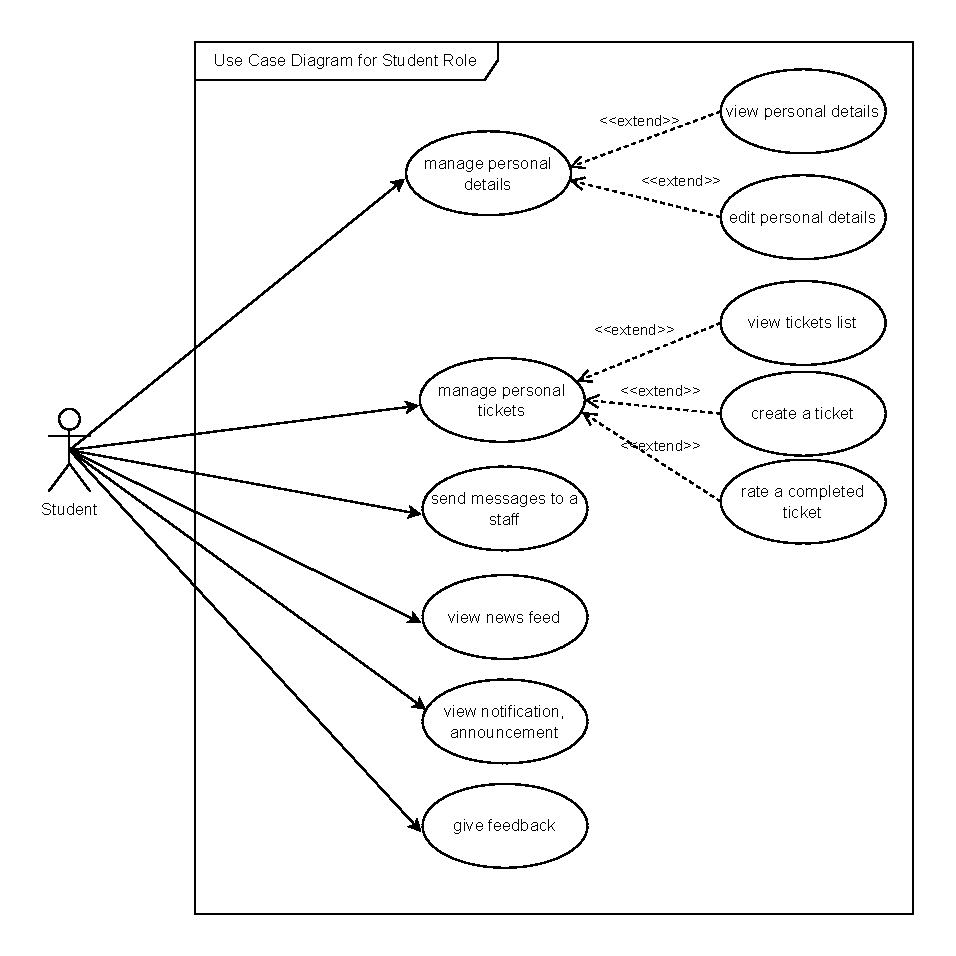
\includegraphics[width=0.82\columnwidth]{graphics/student use case.pdf}
		\caption{Student Use Case Diagram}
		\label{fig:student-use-case}
	\end{figure}
	
	
	
	\begin{figure}[H]
		\centering
		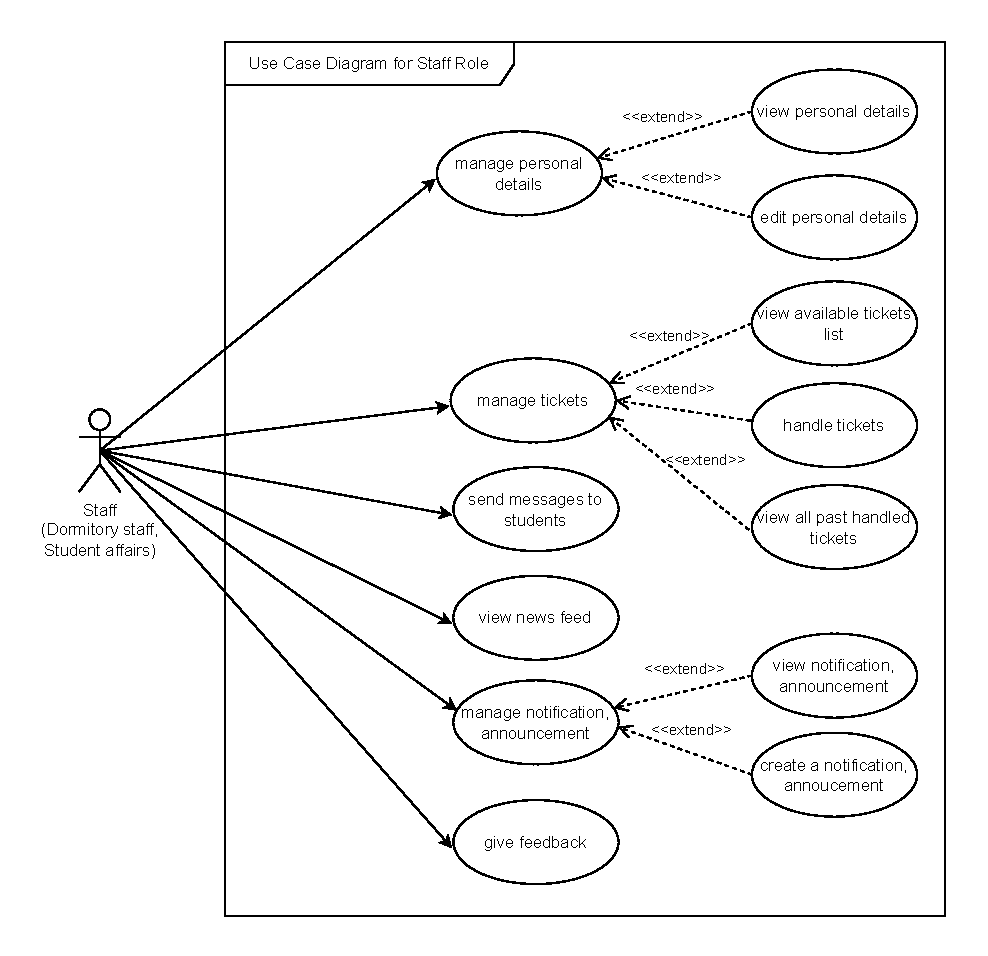
\includegraphics[width=0.9\columnwidth]{graphics/staff use case.pdf}
		\caption{Staff (Dormitory staff, Student affairs) Use Case Diagram}
		\label{fig:staff-use-case}
	\end{figure}
	
	
	
	\begin{figure}[H]
		\centering
		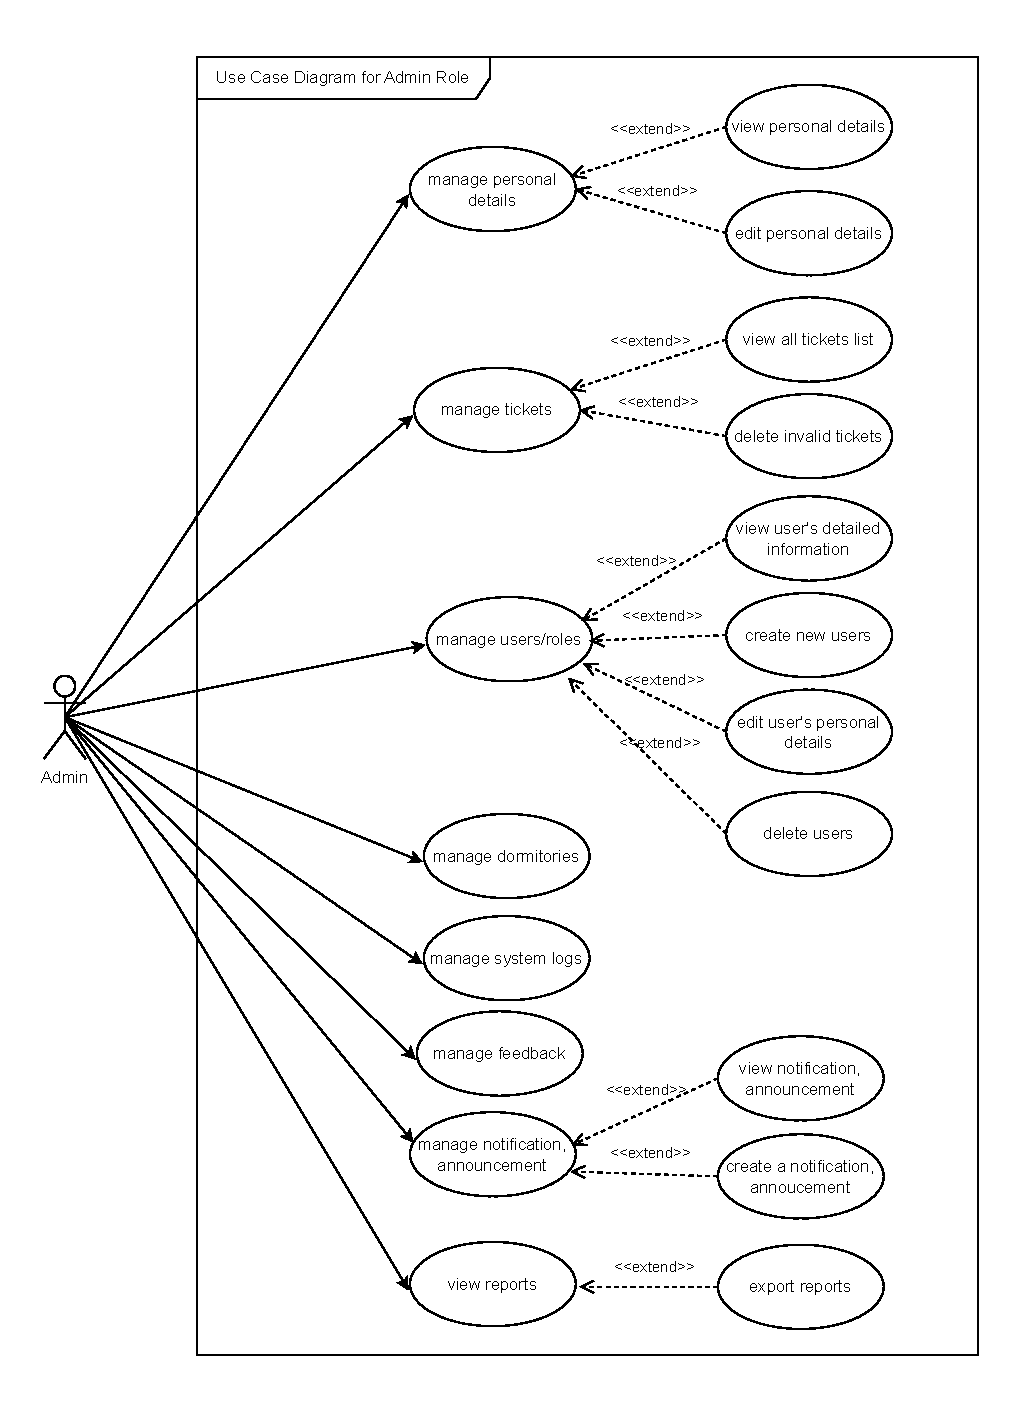
\includegraphics[width=0.84\columnwidth]{graphics/admin-use-case.pdf}
		\caption{Admin Use Case Diagram}
		\label{fig:admin-use-case}
	\end{figure}
	
	
\subsection{Process Workflow Diagrams}	
The core functionality of the Student Life Support Service is its ticket-raising process. The following diagram provides a detailed step-by-step illustration of this process.


\begin{figure}[H]
	\centering
	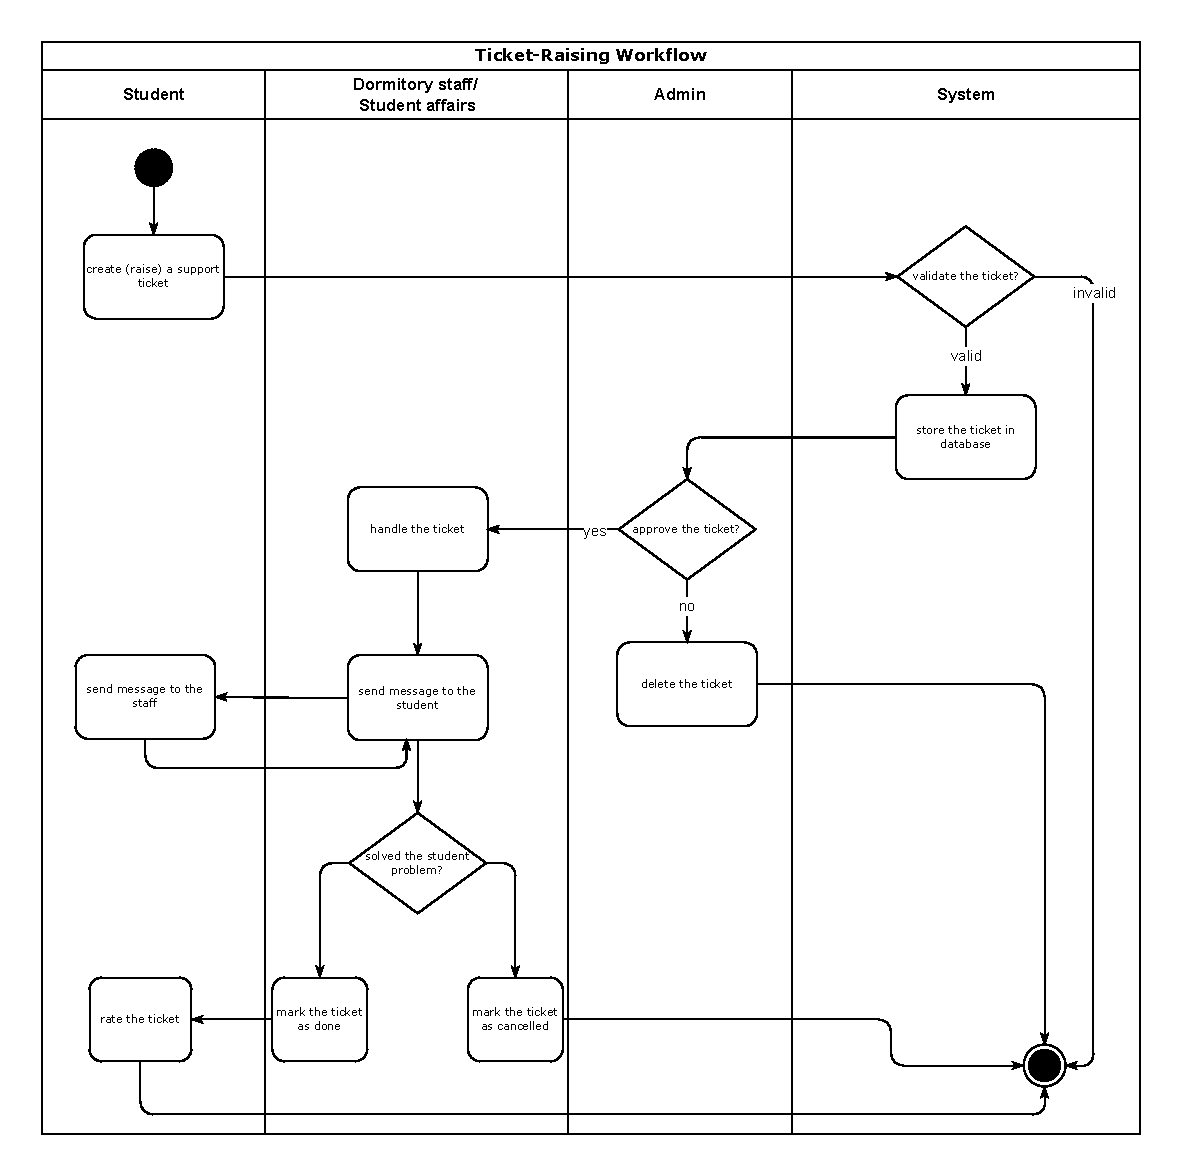
\includegraphics[width=1\columnwidth]{graphics/sys-workflow.pdf}
	\caption{Ticket-Raising Process Workflow}
	\label{fig:ticket-raising-workflow}
\end{figure}


\subsection{Database Design}
	\subsubsection{ER Diagram}
	\begin{figure}[H]
		\centering
		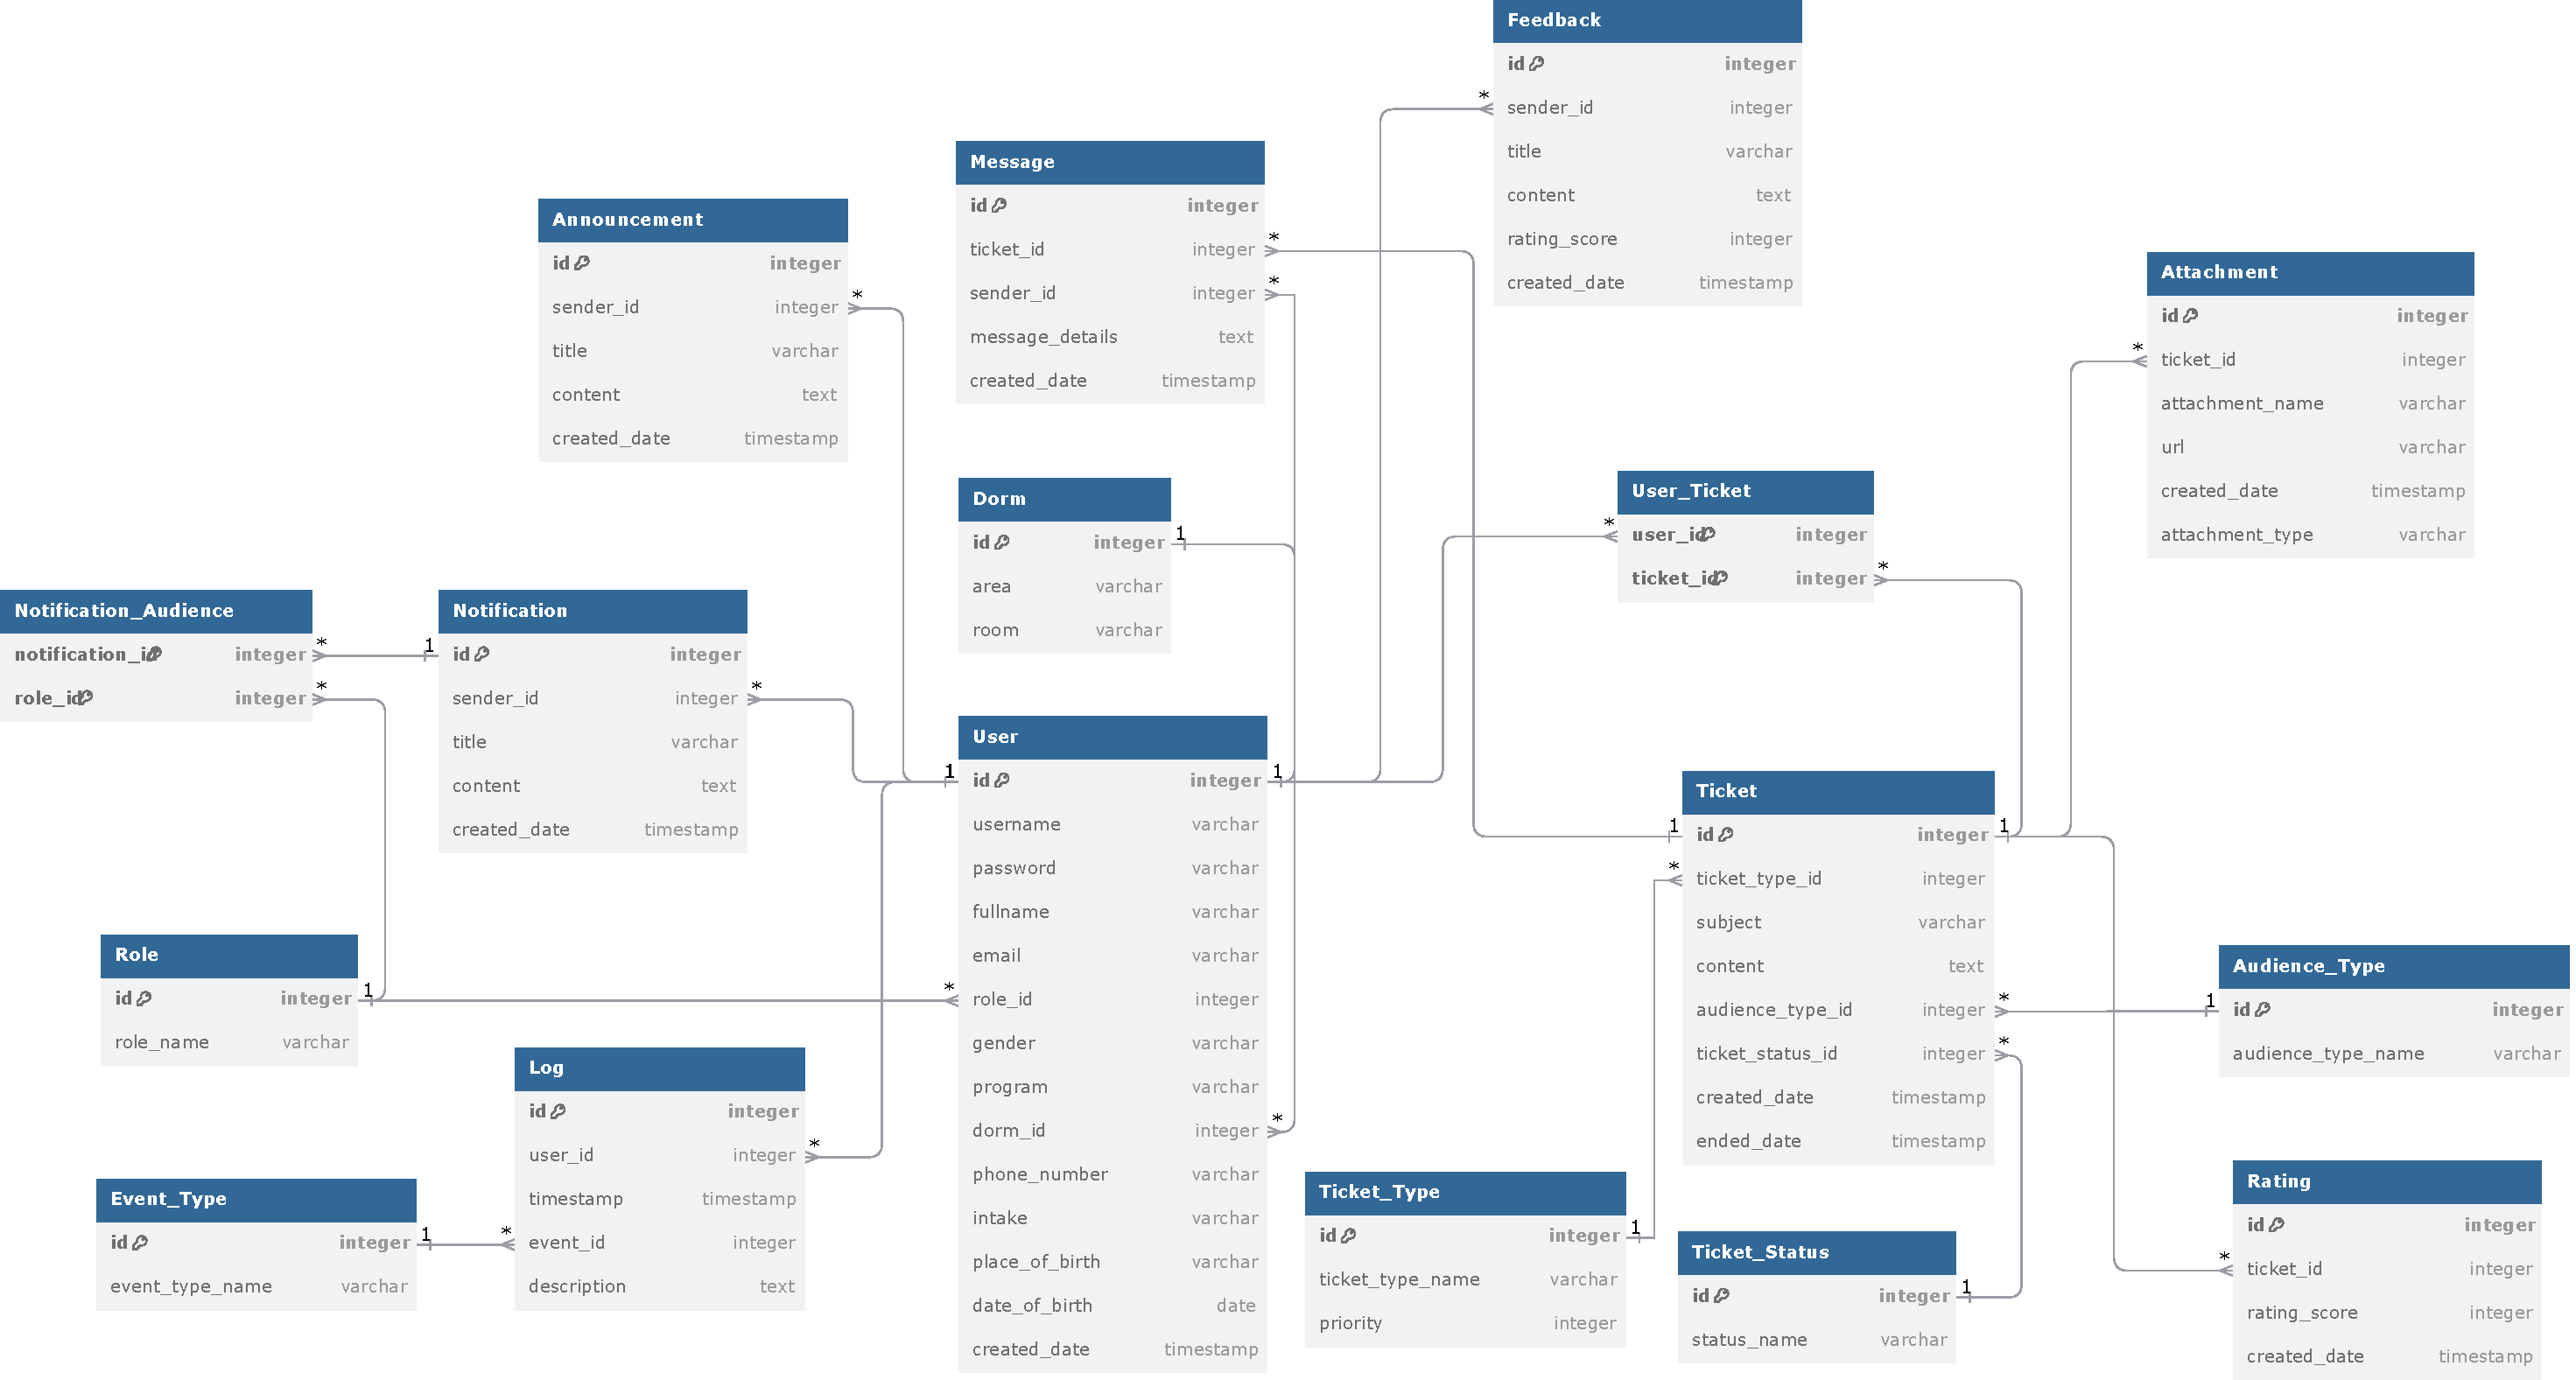
\includegraphics[width=1 \columnwidth]{graphics/er-diagram-v2.pdf}
		\caption{ER Diagram}
		\label{fig:er-diagram}
	\end{figure}


	\subsubsection{User Entity}
%	\newcolumntype{L}{>{\arraybackslash}m{3.5cm}}
	This table presents the essential data required for effective user management, including key details such as username, full name, email, and password (see Table \ref{tab:user-entity})
	
	
	
	\begin{longtable}{|m{1.4cm}|m{2.8cm}|m{2.3cm}|m{2.3cm}|m{7.2cm}|}
		\hline
		\textbf{Key Type} & \textbf{Field Name} & \textbf{Data Type}                                                                                                                            & \textbf{Constraints} & \textbf{Description}   \\ \hline
		\endhead
		
		Primary & id & serial (int) & \makecell[l]{NOT NULL} & id of a user \\ \hline
		 & username & varchar(255) & \makecell[l]{NOT NULL \\ UNIQUE} & the user name of a user, it could be matriculation number of a student \\ \hline
		 & email & varchar(255) & \makecell[l]{NOT NULL \\ UNIQUE} & the email of a user \\ \hline
		 & fullname & varchar(255) & \makecell[l]{NOT NULL} & the full name of a user \\ \hline
		 & gender & varchar(255) & \makecell[l]{NOT NULL} & the gender of a user \\ \hline
		 Foreign & role\_id & int & \makecell[l]{NOT NULL} & the role id of a user \\ \hline
		 Foreign & dorm\_id & int & \makecell[l]{NOT NULL} & the dorm id where user lives (if the user does not live in a dormitory, dorm\_id value equals to 1)\\ \hline
		 & program & varchar(255) &  & the program that user registered at university (E.g: Computer Science, Architecture, etc.)\\ \hline
		 & intake & varchar(255) &  & the time when a user registered a specific program at university (E.g: 2020, 2021, etc.)\\ \hline
		 & phone\_number & varchar(255) & \makecell[l]{NOT NULL} & the phone number of a user\\ \hline
		 & place\_of\_birth & varchar(255) & \makecell[l]{NOT NULL} & the birth place of a user\\ \hline
		 & date\_of\_birth & date & \makecell[l]{NOT NULL} & the birth date of a user\\ \hline
		 & password & varchar(255) & \makecell[l]{NOT NULL} & the password of a user (in hashed string) \\ \hline
		 & created\_date & \makecell[l]{timestamp \\with time \\zone} & NOT NULL & the date time when a user account is created in the system \\ \hline
		 
		
		\caption{User Entity}
		\label{tab:user-entity}
		
	\end{longtable}
	
	
	
	\subsubsection{Ticket Entity}
	This table outlines the key attributes necessary for managing ticket entities within the system. It includes various fields such as the ticket ID, type, subject, content, and associated status. Additionally, it specifies data types, constraints, and a detailed description of each field to ensure proper handling of ticket information (refer to Table \ref{tab:ticket-entity}).
	
	
	
	\begin{longtable}{|m{1.4cm}|m{3.3cm}|m{2.3cm}|m{2.3cm}|m{6.7cm}|}
		\hline
		\textbf{Key Type} & \textbf{Field Name} & \textbf{Data Type}                                                                                                                            & \textbf{Constraints} & \textbf{Description}   \\ \hline
		\endhead
		
		Primary & id & serial (int) & \makecell[l]{NOT NULL} & id of a ticket \\ \hline
		Foreign & ticket\_type\_id & int & \makecell[l]{NOT NULL} & the id of the ticket type \\ \hline
		 & subject & varchar(255) & \makecell[l]{NOT NULL} & the subject (title) the ticket \\ \hline
		 & content & text & \makecell[l]{NOT NULL} & the detailed description of the problem declared in the ticket \\ \hline
		Foreign & audience\_type\_id & int & \makecell[l]{NOT NULL} & the id of audience type assigned to the ticket \\ \hline
		Foreign & ticket\_status\_id & int & \makecell[l]{NOT NULL} & the id of current status assigned to the ticket \\ \hline
		& created\_date & \makecell[l]{timestamp \\with time \\zone} & NOT NULL & the date time when a ticket is created in the system \\ \hline
		& ended\_date & \makecell[l]{timestamp \\with time \\zone} & NOT NULL & the date time when a ticket is marked as done or cancelled in the system \\ \hline
		
		
		\caption{Ticket Entity}
		\label{tab:ticket-entity}
		
	\end{longtable}
	
	
	\subsubsection{User\_Ticket Relationship}
	
		\begin{longtable}{|m{1.4cm}|m{3.3cm}|m{2.3cm}|m{2.3cm}|m{6.7cm}|}
			\hline
			\textbf{Key Type} & \textbf{Field Name} & \textbf{Data Type}                                                                                                                            & \textbf{Constraints} & \textbf{Description}   \\ \hline
			\endhead
			
			Primary & user\_id & int & \makecell[l]{NOT NULL} & id of a ticket \\ \hline
			
			Primary & ticket\_id & int & \makecell[l]{NOT NULL} & id of a user \\ \hline

			\caption{User\_Ticket Relationship}
			\label{tab:user-ticket}
			
		\end{longtable}
		
		This table describes the relationship between users and tickets within the system. It contains two primary key fields: \texttt{user\_id} and \texttt{ticket\_id}, each identified by a unique integer. The \texttt{user\_id} represents the unique identifier for a user, while the \texttt{ticket\_id} corresponds to a unique ticket within the system. Both fields are non-nullable, ensuring that each user and ticket association is properly recorded and maintained (refer to Table \ref{tab:user-ticket}). This relationship is essential for tracking which users have raised and handled specific tickets in the system .
	
	
	\subsubsection{Ticket\_Type Entity}
	
	\begin{longtable}{|m{1.4cm}|m{3.3cm}|m{2.3cm}|m{2.3cm}|m{6.7cm}|}
		\hline
		\textbf{Key Type} & \textbf{Field Name} & \textbf{Data Type}                                                                                                                            & \textbf{Constraints} & \textbf{Description}   \\ \hline
		\endhead
		
		Primary & id & serial (int) & \makecell[l]{NOT NULL} & id of a ticket type \\ \hline
		 & ticket\_type\_name & varchar(255) & \makecell[l]{NOT NULL \\ UNIQUE} & the type name of a ticket \\ \hline
		
		& priority & int & \makecell[l]{NOT NULL} & the priority of the ticket type (higher indicates lower priority) \\ \hline
		
		\caption{Ticket\_Type Entity}
		\label{tab:ticket-type}
		
	\end{longtable}
	
	This table defines the Ticket\_Type entity, which represents various types of tickets that can be created within the system. It consists of three fields:
%	
%	The id field, which is a primary key, represented as a serial integer, serving as the unique identifier for each ticket type.
%	
%	The \texttt{ticket\_type\_name} field, stored as a \texttt{varchar(255)}, holds the name of the ticket type, such as "Technical Issue" or "Academic Inquiry."
	
%	The priority field, an integer, determines the urgency level of the ticket type, where a higher number indicates lower priority.
	\begin{itemize}
		\item The \texttt{id} field, which is a primary key, represented as a serial integer, serving as the unique identifier for each ticket type.
		
		\item The \texttt{ticket\_type\_name} field, stored as a \texttt{varchar(255)}, holds the name of the ticket type, such as "Lost items" or "Harassment".
		
		\item The \texttt{priority} field, an integer, determines the urgency level of the ticket type, where a higher number indicates lower priority.
	\end{itemize}
	
	\noindent All fields are marked as \texttt{NOT NULL}, ensuring that every ticket type has a unique identifier, name, and priority level. This structure is essential for organizing and managing different categories of support tickets in the system (refer to Table \ref{tab:ticket-type}).
	
	
	
	\subsubsection{Ticket\_Status Entity}
	
	\begin{longtable}{|m{1.4cm}|m{3.3cm}|m{2.3cm}|m{2.3cm}|m{6.7cm}|}
		\hline
		\textbf{Key Type} & \textbf{Field Name} & \textbf{Data Type}                                                                                                                            & \textbf{Constraints} & \textbf{Description}   \\ \hline
		\endhead
		
		Primary & id & serial (int) & \makecell[l]{NOT NULL} & id of a ticket status \\ \hline
		& status\_name & varchar(255) & \makecell[l]{NOT NULL \\ UNIQUE} & the status name of a ticket \\ \hline
		
		\caption{Ticket\_Status Entity}
		\label{tab:ticket-status}
		
	\end{longtable}
	
	
	This table describes the Ticket\_Status entity, which is used to represent the current status of a support ticket within the system. It contains two fields:
	
	
	\begin{enumerate}
		
		\item The \texttt{id} field is the primary key, defined as a serial integer, serving as the unique identifier for each ticket status. This field is essential for distinguishing between different statuses.
		
		\item The \texttt{status\_name} field is a \texttt{varchar(255)} that stores the name of the ticket status, such as "pending," "in progress," "done," or "cancelled." These status names provide insight into the progress of each support ticket.
	\end{enumerate}
	
	\noindent Both fields are marked as \texttt{NOT NULL}, ensuring that every ticket status has a unique identifier and name, which is crucial for tracking and managing the lifecycle of tickets (refer to Table \ref{tab:ticket-status}).
	
	
	
	\subsubsection{Audience\_Type Entity}
	
	\begin{longtable}{|m{1.4cm}|m{3.8cm}|m{2.3cm}|m{2.3cm}|m{6.2cm}|}
		\hline
		\textbf{Key Type} & \textbf{Field Name} & \textbf{Data Type}                                                                                                                            & \textbf{Constraints} & \textbf{Description}   \\ \hline
		\endhead
		
		Primary & id & serial (int) & \makecell[l]{NOT NULL} & id of a ticket audience type \\ \hline
		& audience\_type\_name & varchar(255) & \makecell[l]{NOT NULL \\ UNIQUE} & the target audience type name of a ticket \\ \hline
		
		\caption{Audience\_Type Entity}
		\label{tab:audience-type}
		
	\end{longtable}
	
	
	This table outlines the Audience\_Type entity, which is used to categorize the audience for support tickets within the system. It includes two fields:
	
	\begin{itemize}
		\item The \texttt{id} field, which is the primary key, is a serial integer that uniquely identifies each audience type. This field ensures each audience type is distinct and traceable.
		
		\item The \texttt{audience\_type\_name} field is a \texttt{varchar(255)} that stores the name of the audience type for a ticket. It could be either "private" or "public," where public tickets are visible to other students, while private tickets are only visible to the ticket creator and assigned staff.
	\end{itemize}
	

	\noindent Both fields are defined as NOT NULL, ensuring that each audience type has a unique identifier and a clearly defined type name, which is essential for managing ticket visibility (refer to Table \ref{tab:audience-type}).
	
	
	
	\subsubsection{Attachment Entity}
	
	\begin{longtable}{|m{1.4cm}|m{3.3cm}|m{2.3cm}|m{2.3cm}|m{6.3cm}|}
		\hline
		\textbf{Key Type} & \textbf{Field Name} & \textbf{Data Type}                                                                                                                            & \textbf{Constraints} & \textbf{Description}   \\ \hline
		\endhead
		
		Primary & id & serial (int) & \makecell[l]{NOT NULL} & id of an attachment \\ \hline
		Foreign & ticket\_id & int & \makecell[l]{NOT NULL} & the reference ticket id which has an attachment \\ \hline
		 & attachment\_name & varchar(255) & \makecell[l]{NOT NULL} & the original name of the attachment \\ \hline
		 & url & varchar(255) & \makecell[l]{NOT NULL \\ UNIQUE} & the address of an attachment on the server  \\ \hline
		 & created\_date & \makecell[l]{timestamp \\with time \\zone} & NOT NULL & the date time when an attachment is firstly uploaded to the system \\ \hline
		
		\caption{Attachment Entity}
		\label{tab:attachment}
		
	\end{longtable}
	
	The Attachment entity captures essential details about files associated with support tickets in the system. The table comprises the following key fields:
	
	\begin{itemize}
		\item \texttt{id}: This primary key is a serial integer that uniquely identifies each attachment in the system, ensuring every file is traceable.
		
		\item \texttt{ticket\_id}: A foreign key linking the attachment to the specific ticket it belongs to, creating a clear relationship between files and their corresponding support tickets.
		
		\item \texttt{attachment\_name}: This field stores the original name of the file, providing users and administrators with a clear reference to the document.
		
		\item \texttt{url}: A \texttt{varchar(255)} field that holds the unique server address where the attachment is stored. It is constrained to be both \texttt{NOT NULL} and \texttt{UNIQUE}, ensuring each file is stored at a distinct location.
		
		\item \texttt{created\_date}: A timestamp with time zone that records the exact moment the attachment was uploaded to the system, offering important chronological information for ticket management.
	\end{itemize}

	\noindent This entity provides a robust structure for managing files, enabling easy access and secure storage of attachments related to user support requests (refer to Table \ref{tab:attachment}).
	
	
	
	\subsubsection{Rating Entity}
	
	\begin{longtable}{|m{1.4cm}|m{2.5cm}|m{2.3cm}|m{2.3cm}|m{6.7cm}|}
		\hline
		\textbf{Key Type} & \textbf{Field Name} & \textbf{Data Type}                                                                                                                            & \textbf{Constraints} & \textbf{Description}   \\ \hline
		\endhead
		
		Primary & id & serial (int) & \makecell[l]{NOT NULL} & id of a rating \\ \hline
		Foreign & ticket\_id & int & \makecell[l]{NOT NULL} & the reference ticket id which has the rating \\ \hline
		& rating\_score & int & \makecell[l]{NOT NULL} & the rating score of a ticket \\ \hline
		& created\_date & \makecell[l]{timestamp \\with time \\zone} & NOT NULL & the date time when user rates a ticket. \\ \hline
		
		\caption{Rating Entity}
		\label{tab:rating}
		
	\end{longtable}
	
	The Rating entity is designed to capture and store feedback from users regarding their support tickets. This table includes several key fields:
	
	\begin{itemize}
		\item \texttt{id}: A serial integer serving as the primary key, which uniquely identifies each rating entry in the system.
		
		\item \texttt{ticket\_id}: A foreign key that links the rating to the specific ticket being evaluated, ensuring that every rating is associated with a particular support request.
		
		\item \texttt{rating\_score}: A number field that holds the actual score or feedback provided by the user. This score reflects the user's level of satisfaction with the handling of their ticket.
		
		\item \texttt{created\_date}: A timestamp with time zone indicating when the rating was submitted, allowing for tracking and auditing of feedback over time.
	\end{itemize}
	
	\noindent This entity is crucial for maintaining a structured and traceable system for user feedback, enabling continuous service improvement based on user satisfaction (refer to Table \ref{tab:rating}).
	
	
	
	\subsubsection{Feedback Entity}
	
	\begin{longtable}{|m{1.4cm}|m{2.5cm}|m{2.3cm}|m{2.3cm}|m{6.7cm}|}
		\hline
		\textbf{Key Type} & \textbf{Field Name} & \textbf{Data Type}                                                                                                                            & \textbf{Constraints} & \textbf{Description}   \\ \hline
		\endhead
		
		Primary & id & serial (int) & \makecell[l]{NOT NULL} & id of a feedback \\ \hline
		Foreign & sender\_id & int & \makecell[l]{NOT NULL} & the id of the user who gives the feedback \\ \hline
		& title & varchar(255) & \makecell[l]{NOT NULL} & the title (subject) of the feedback \\ \hline
		& content & text & \makecell[l]{NOT NULL} & the details of the feedback \\ \hline
		& rating\_score & int & \makecell[l]{NOT NULL} & the rating score of the feedback \\ \hline
		& created\_date & \makecell[l]{timestamp \\with time \\zone} & NOT NULL & the date time when user gives the feedback. \\ \hline
		
		\caption{Feedback Entity}
		\label{tab:feedback}
		
	\end{longtable}
	
	The Feedback entity is structured to store user feedback, enabling users to provide detailed evaluations of the system. It consists of several key fields:
	
	\begin{itemize}
		\item \texttt{id}: A serial integer that serves as the primary key, uniquely identifying each feedback entry.
		
		\item \texttt{sender\_id}: A foreign key representing the user who submits the feedback, ensuring proper linkage between the feedback and its author.
		
		\item \texttt{title}: A \texttt{varchar(255)} field that contains the subject or title of the feedback, summarizing the main point of the user's input.
		
		\item \texttt{content}: A text field used for the detailed explanation of the feedback, where users can elaborate on their experience or suggestions.
		
		\item \texttt{rating\_score}: An integer representing the overall rating score associated with the feedback, allowing users to quantify their level of satisfaction.
		
		\item \texttt{created\_date}: A timestamp with time zone capturing when the feedback was submitted, which aids in tracking and analysis over time.
	\end{itemize}
	
	\noindent This entity is critical for gathering and storing user insights, helping administrators to improve the system based on user evaluations and suggestions (refer to Table \ref{tab:feedback}).
	
	
	
	\subsubsection{Message Entity}
	
	\begin{longtable}{|m{1.4cm}|m{2.9cm}|m{2.3cm}|m{2.3cm}|m{6.7cm}|}
		\hline
		\textbf{Key Type} & \textbf{Field Name} & \textbf{Data Type}                                                                                                                            & \textbf{Constraints} & \textbf{Description}   \\ \hline
		\endhead
		
		Primary & id & serial (int) & \makecell[l]{NOT NULL} & id of a message \\ \hline
		Foreign & ticket\_id & int & \makecell[l]{NOT NULL} & the id of a ticket which has the message (acts as a conversation id) \\ \hline
		& sender\_id & int & \makecell[l]{NOT NULL} & id of a user who has the message \\ \hline
		& message\_details & text & \makecell[l]{NOT NULL} & the details of a message \\ \hline
		& created\_date & \makecell[l]{timestamp \\with time \\zone} & NOT NULL & the date time when user send a message. \\ \hline
		
		\caption{Message Entity}
		\label{tab:message}
		
	\end{longtable}
	
	
	
	The Message entity is designed to store and manage the communication between users related to a specific ticket, acting as the foundation for the system's real-time messaging feature. The key components of this entity include:
	
	\begin{itemize}
		\item \texttt{id}: A serial integer that uniquely identifies each message, serving as the primary key.
		
		\item \texttt{ticket\_id}: A foreign key that links the message to a specific ticket, representing the conversation associated with that ticket.
		
		\item \texttt{sender\_id}: This field stores the id of the user who sent the message, ensuring proper identification of the sender.
		
		\item \texttt{message\_details}: A text field that contains the content of the message, capturing the full details of the communication.
		
		\item \texttt{created\_date}: A timestamp with time zone that records when the message was sent, which helps in tracking the conversation timeline.
	\end{itemize}
	
	\noindent This entity is essential for facilitating and managing user interactions within the system's ticketing process, ensuring seamless communication between users (refer to Table \ref{tab:message}).
	
	
	

\subsection{System Architecture}

The system follows a three-tier architecture, consisting of the following layers:

\begin{figure}[H]
	\centering
	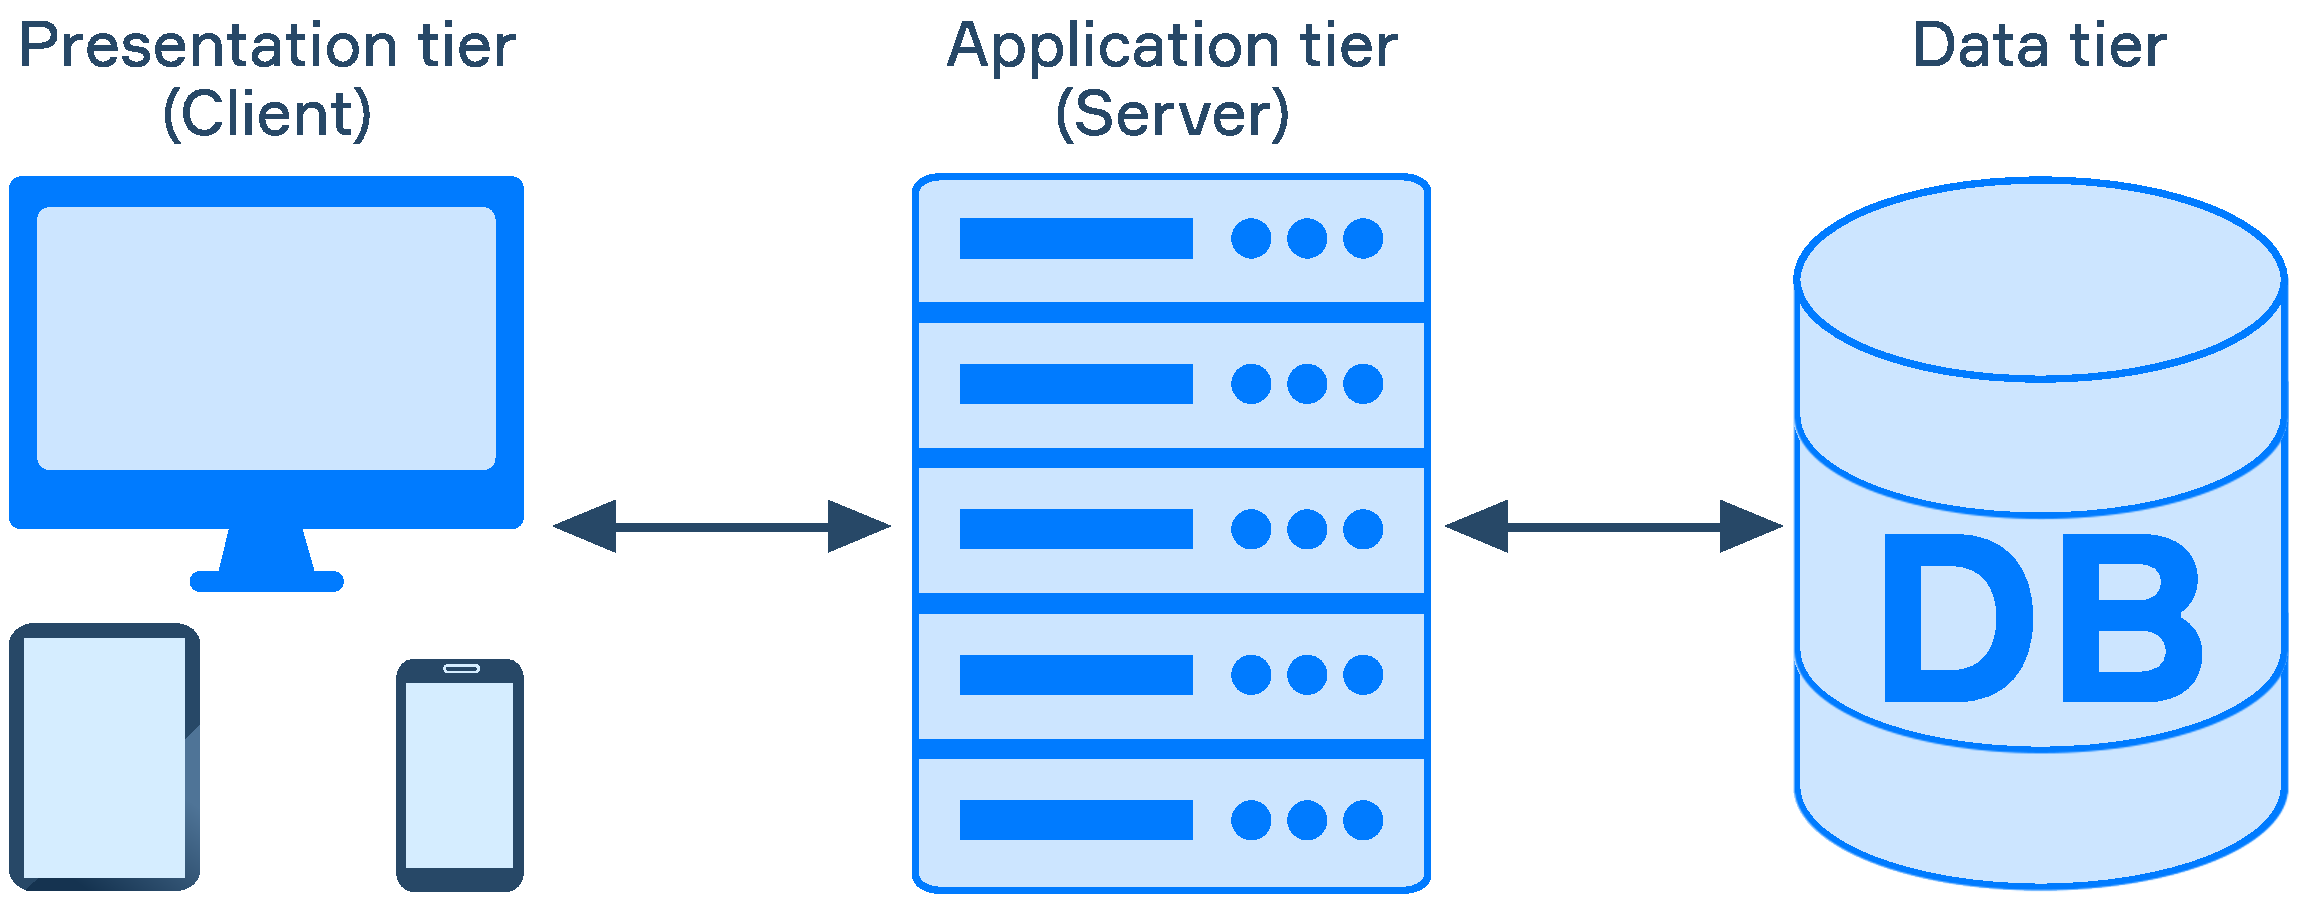
\includegraphics[width=0.7\columnwidth]{graphics/3-tier-arch.pdf}
	\caption{Three-tier Architecture \cite{3-tier}}
	\label{fig:3-tier}
\end{figure}


\begin{enumerate}
	\item \textbf{Presentation Layer (Client):}
	
	Handles all interactions with the user.
	Implements the user interface using ReactJS and Material UI.
	Communicates with the server through RESTful API calls and SocketIO for real-time features.
	Responsible for rendering components, collecting user input, and displaying data received from the backend.
	
	\item \textbf{Business Logic Layer (Server)}:
	
	NodeJS and ExpressJS handle the core business logic, such as processing support ticket requests, authenticating users, managing roles, and communicating with the database.
	SocketIO is used to manage real-time messaging between students and staff.
	Implements security features like JWT-based authentication and session management using Redis.
	
	\item \textbf{ Data Layer (Database)}:
	
	PostgreSQL stores all persistent data, including user profiles, support tickets, messages, and system logs.
	The server communicates with the database using SQL queries to retrieve, create, update, and delete records.
	Ensures data consistency and integrity by enforcing constraints, foreign keys, and relationships.
	
\end{enumerate}


\subsection{Frontend Design}












%	
	


	